% !TEX root = ../main.tex
\subsubsection{Geometry Effect}
\label{12.42::geometry_effect}
    To evaluate the enhancement in vertex resolution, we will compare the vertex positions of tracks that underwent only DC reconstruction with those that underwent both DC and FMT reconstruction.
    For convenience, we will refer to the former as DC tracks and the latter as FMT tracks.
    Considering that the $z$ axis is aligned with the beamline, Figure \ref{fig::12.41::dc_vs_fmt_vz_11983} illustrates the $z$ positions of the vertex for DC tracks versus FMT tracks.

    To comprehend the plot in Figure \ref{fig::12.41::dc_vs_fmt_vz_11983}, it is valuable to examine the RG-F target.
    The target consists of a large gas-filled chamber with a varying composition across different runs.
    The distance between the chamber windows measures $553.32$ millimetres.
    Furthermore, it was observed that the upstream window of the target is positioned approximately $24$ millimetres away from the beam window.
    All windows are constructed from aluminium and have a thickness of $15$ micrometers.
    A detailed depiction of the target can be found in Addendum 1.

    Based on Figure \ref{fig::12.41::dc_vs_fmt_vz_11983}, it is evident that the FMT detector solely detects the upstream windows, completely overlooking the downstream one.
    This issue stems from a geometric constraint: the downstream window falls outside the active detection area of the FMT.
    This effect is clearly illustrated in Figure \ref{eq::12.42::vz_vs_theta}, where the $\theta$ angle is plotted against the vertex $z$ coordinate.
    The two red lines in the plots represent the FMT's active area, and it is apparent that the downstream window lies outside this region, thereby explaining its absence.

    \begin{figure}[t!]
        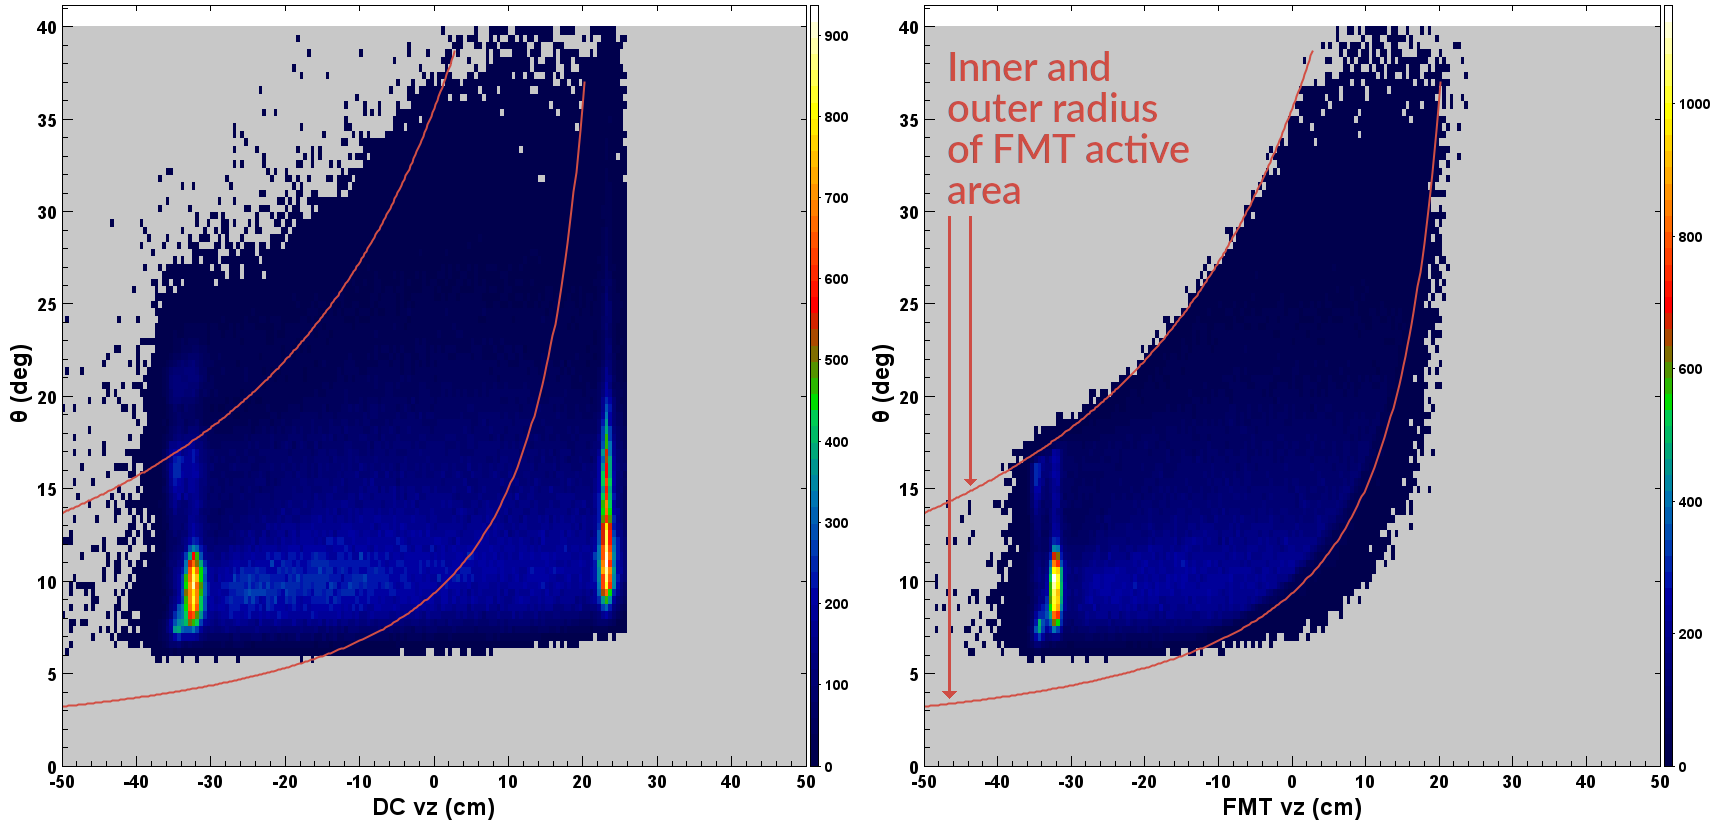
\includegraphics[scale=0.24]{42theta_dc_vs_fmt.png}
        \caption[$z$ vs. $\theta$ for DC and FMT]
        {$z$ vs. $\theta$ for DC and FMT for electrons without any geometry correction.
        FMT's active area are shown in red lines.}
        \floatfoot{Source: Own elaboration, using the \texttt{fmtVertex.groovy} script in \href{https://github.com/JeffersonLab/clas12alignment}{CLAS12 alignment software}.}
        \label{eq::12.42::vz_vs_theta}
    \end{figure}

    To compensate for this geometric effect, we introduce an additional cut based on the plotted curves.
    The curves can be described by the following equations
    \begin{equation}
        c_1(z) = 57.29 \cdot \arctan\left(\frac{r_\text{inner}}{z_0 - z}\right),
        \hspace{0.5cm}
        c_2(z) = 57.29 \cdot \arctan\left(\frac{r_\text{outer}}{z_0 - z}\right).
        \label{eq::12.42::fmt_geometry_cut}
    \end{equation}

    Here, $r_\text{inner}$ represents the radius of the hole at the center of the FMT, $r_\text{outer}$ denotes the radius of the outer circumference of the FMT, and $z_0$ corresponds to the $z$ position of the first FMT layer plus the drift distance.
    All these parameters are obtained from the CCDB.
